\chapter{Graphrepräsentationen von Bildern}
\label{graphrepraesentationen_von_bildern}

Als eine \emph{Graphrepräsentation eines Bildes} $\gls{B} \in \gls{R}^{H \times W \times C}$ wird eine Darstellung von \gls{B} als ein gewichteter, ungerichteter sowie schleifenloser Graph \gls{G} verstanden, deren Knoten Informationen zu ausgewählten Bereichen von \gls{B} über eine Merkmalsmatrix $\gls{F} \in \gls{R}^{N \times M}$ speichern und deren Kanten eine Aussage über die örtlichen Nachbarschaften eines jeden Bildbereichs innewohnt.
Formal lässt sich eine Graphrepräsentation eines Bildes damit als ein \emph{Graph im zweidimensionalen euklidischen Raum} $\gls{G} = \left(\gls{V}, \gls{E}, \gls{p}\right)$ verstehen, dem zusätzlich zu seinen Knoten- und Kantenmengen anstatt einer Gewichtsfunktion $\gls{w} \colon \gls{V} \times \gls{V} \to \gls{R}$ eine Positionsfunktion $\gls{p} \colon \gls{V} \to \gls{R}^2$ auf seinen Knoten in den zweidimensionalen euklidischen Raum $\gls{R}^2$ zugeordnet ist.
Das Gewicht $\gls{w} \colon \gls{E} \to \left[0, 1\right]$ einer Kante ergibt sich dann implizit als \enquote{Abstandsfunktion} mit Hilfe der euklidischen Norm $\left\|\cdot\right\|_2$ auf den Positionen der Knoten und der Gaußfunktion als
\begin{equation}
  \gls{w}\left(\gls{v}_i, \gls{v}_j\right) \coloneqq \begin{cases}
    \exp\left(-\frac{\left\|\gls{p}\left(\gls{v}_i\right) - \gls{p}\left(\gls{v}_j\right)\right\|_2^2}{2\gls{sigma}^2}\right), & \text{wenn }\left(\gls{v}_i, \gls{v}_j\right) \in \gls{E},\\
    0, & \text{sonst}
  \end{cases}
  \label{eq:gauss}
\end{equation}
mit der Standardabweichung $\gls{sigma} \in \gls{R}$~\cite{Shuman}.
Abbildung~\ref{fig:gauss} veranschaulicht die Gewichtsfunktion anhand unterschiedlich gewählter $\gls{sigma}$.
\begin{figure}[t]
\centering
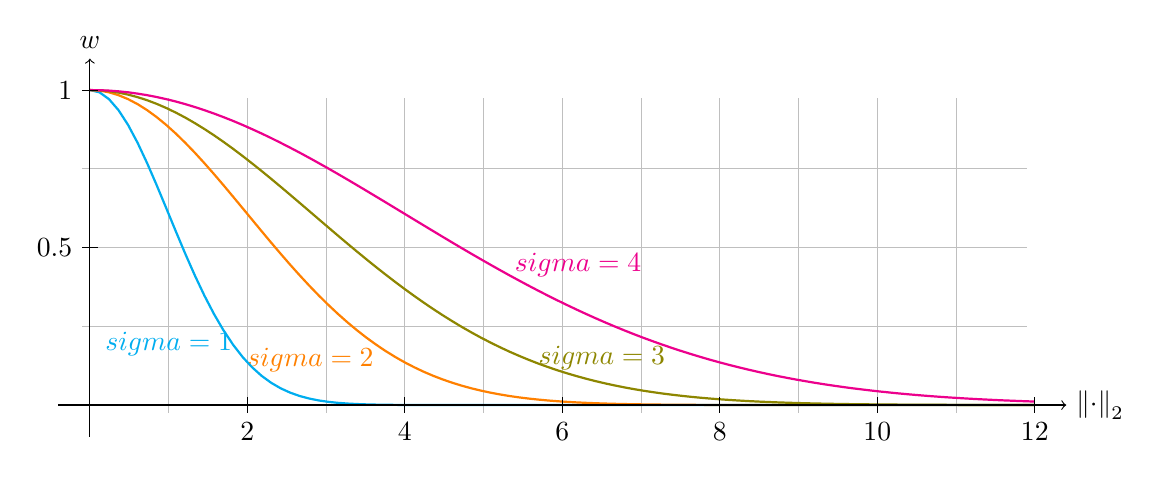
\begin{tikzpicture}
  \draw[color=lightgray] (-0.1, -0.1) grid (11.9, 3.9);
  \tikzstyle{color1}=[color=cyan]
  \tikzstyle{color2}=[color=orange]
  \tikzstyle{color3}=[color=olive]
  \tikzstyle{color4}=[color=magenta]

  \draw[color1] (1,0.5) node[above]   {$\gls{sigma} = 1$};
  \draw[color2] (2.8,0.3) node[above] {$\gls{sigma} = 2$};
  \draw[color3] (6.5,0.32) node[above] {$\gls{sigma} = 3$};
  \draw[color4] (6.2,1.5) node[above] {$\gls{sigma} = 4$};

  \draw [color1, thick,domain=0:12, samples=100] plot (\x,4*exp{-(\x)^2/2});  % 1
  \draw [color2, thick,domain=0:12, samples=100] plot (\x,4*exp{-(\x)^2/8});  % 2
  \draw [color3, thick,domain=0:12, samples=100] plot (\x,4*exp{-(\x)^2/16});  % 3
  \draw [color4, thick,domain=0:12, samples=100] plot (\x,4*exp{-(\x)^2/32});  % 4

  \draw[->] (-0.4, 0) -- (12.4, 0) node[right] {${\left\|\cdot\right\|}_2$};
  \draw[->] (0, -0.4) -- (0, 4.4) node[above] {$w$};
  \draw (0.1, 2) -- (-0.1, 2) node[left] {$0.5$};
  \draw (0.1, 4) -- (-0.1, 4) node[left] {$1$};
  \draw (2, 0.1) -- (2, -0.1) node[below] {$2$};
  \draw (4, 0.1) -- (4, -0.1) node[below] {$4$};
  \draw (6, 0.1) -- (6, -0.1) node[below] {$6$};
  \draw (8, 0.1) -- (8, -0.1) node[below] {$8$};
  \draw (10, 0.1) -- (10, -0.1) node[below] {$10$};
  \draw (12, 0.1) -- (12, -0.1) node[below] {$12$};

\end{tikzpicture}
  \caption[Kantengewichtsberechnung über Gaußfunktion]{Illustration der \enquote{invertierten} Kantengewichte $w \in \left[0, 1\right]$ basierend auf dessen Länge, gegeben durch die euklidische Norm ${\left\|\cdot\right\|}_2$.
  Je größer $\gls{sigma} \in \gls{R}$ gewählt, umso \enquote{stumpfer} zeichnet sich die Gaußfunktion und umso längere Kanten erhalten ein Gewicht $\gg 0$.
  Die Wahl von \gls{sigma} ist damit abhängig von der Ausdehnung der Distanzen eines Graphen.}
\label{fig:gauss}
\end{figure}

Aufgrund der Symmetrie von ${\left\|\cdot\right\|}_2$ folgt insbesondere sofort die Ungerichtheit des Graphen \gls{G}, \dhe{} $\gls{w}\left(\gls{v}_i, \gls{v}_j\right) = \gls{w}\left(\gls{v}_j, \gls{v}_i\right)$.
Die Gaußfunktion \enquote{invertiert} dabei den Abstand zweier Knoten zueinander, sodass Knoten die weiter voneinander entfernt liegen ein geringeres Gewicht besitzen.
Das korrespondiert mit dem üblichen Verständnis eines Kantengewichts in Graphen.
Knoten, die näher am Ursprungsknoten liegen, gelten als \enquote{wichtiger} und bekommen deshalb ein größeres Gewicht.
Insbesondere stimmt dies mit der Konvention überein, dass $\gls{w}\left(\gls{v}_i, \gls{v}_j\right) = 0$ für $\left(\gls{v}_i, \gls{v}_j\right) \notin \gls{E}$.
Damit lässt sich weiterhin die korrespondierende Adjazenzmatrix $\gls{Adist} \in \left[0, 1\right] \in \gls{R}^{N \times N}$ wie bekannt mit ${\left(\gls{Adist}\right)}_{ij} \coloneqq \gls{w}\left(\gls{v}_i, \gls{v}_j\right)$ definieren.

Zusätzlich zu dem Abstand der Knoten \bzw{} der Länge der Kanten eines Graphen im zweidimensionalen euklidischen Raum $\gls{G} = \left(\gls{V}, \gls{E}, \gls{p}\right)$ lassen sich die Ausrichtungen der Kanten über die Positionen der Knoten von \gls{G} festhalten.
Aus $\gls{p} \colon \gls{V} \to \gls{R}^2$ wird folglich über
\begin{equation}
  \gls{winkel}\left(\gls{v}_i, \gls{v}_j\right) \coloneqq \begin{cases}
    \mathrm{atan2}\left({\gls{p}\left(\gls{v}_j\right)}_1 - {\gls{p}\left(\gls{v}_i\right)}_1, {\gls{p}\left(\gls{v}_j\right)}_2 - {\gls{p}\left(\gls{v}_i\right)}_2\right) + \pi, & \text{wenn }\left(\gls{v}_i, \gls{v}_j\right) \in \gls{E},\\
    0, & \text{sonst}
  \end{cases}
  \label{eq:winkelfunktion}
\end{equation}
eine \emph{Winkelfunktion} $\gls{winkel} \colon \gls{V} \times \gls{V} \to \left[0, 2\pi\right]$ auf den Kanten von \gls{G} im Uhrzeigersinn definiert, wobei $\mathrm{atan2}\left(x, y\right) \in \left[-\pi, \pi\right]$ den Arkustangens von $x/y$ berechnet, aber im Gegensatz zu $\mathrm{atan}\left(\cdot\right)$ die Vorzeichen beider Parameter beachtet und so den Quadranten des Ergebnisses bestimmen kann (\vgl{}~\cite{atan2}).
Der Winkel Null wird dabei explizit als $2\pi$ definiert, sodass weiterhin $\gls{winkel}\left(\gls{v}_i, \gls{v}_j\right) = 0$ gilt, falls $\left(\gls{v}_i, \gls{v}_j\right) \notin \gls{E}$.
Analog zu \gls{Adist} lässt sich damit die Adjazenzmatrix $\gls{Arad} \in {\left[0, 2\pi\right]}^{N \times N}$ mit ${\left(\gls{Arad}\right)}_{ij} \coloneqq \gls{winkel}\left(\gls{v}_i, \gls{v}_j\right)$ definieren.
Es ist anzumerken, dass die Winkelfunktion \gls{winkel} im Gegensatz zur Gewichtsfunktion \gls{w} nicht symmetrisch \bzw{} ungerichtet ist, \dhe{} $\gls{winkel}\left(\gls{v}_i, \gls{v}_i\right) \neq \gls{winkel}\left(\gls{v}_j, \gls{v}_i\right)$.
Insbesondere definiert \gls{Arad} damit einen gerichteten Graphen.

Die beiden Adjazenzmatrizen \gls{Adist} und \gls{Arad} beschreiben den Graphen $\gls{G} = \left(\gls{V}, \gls{E}, \gls{p}\right)$ bis auf Translation eindeutig.
Eine Veränderung einer Position $\gls{p}\left(\gls{v}\right)$ eines Knotens $\gls{v} \in \gls{V}$ führt sowohl zu einer Veränderung in \gls{Adist} als auch in \gls{Arad}.
Eine Translation aller Knoten um $\ve{\delta} \in \gls{R}^2$, \dhe{} $\gls{p}\left(\gls{v}\right) \rightarrow \gls{p}\left(\gls{v}\right) + \ve{\delta}$, generiert hingegen vollkommen äquivalente Adjazenzmatrizen \gls{Adist} sowie \gls{Arad}.
In der Regel ist dies kein Nachteil, denn nur in den seltensten Fällen interessieren uns die absoluten Positionen der Knoten in \gls{G}, wohingegen der Abstand und die Ausrichtungen der Knoten zueinander eine größere Bedeutung genießen.

Im Folgenden werden basierend auf der Definition eines Graphen im zweidimensionalen  euklidischen Raum zwei Ansätze für eine Graphrepräsentation von Bildern vorgestellt — der Repräsentation über ein reguläres Gitter sowie der Repräsentation über die Bestimmung von Superpixeln eines Bildes.

\section{Gitter}
\label{gitter}

Die einfachste Form einer Graphrepräsentation \gls{G} eines Bildes $\gls{B} \in \gls{R}^{H \times W \times C}$ ist die Repräsentation des Bildes über einen regulären Gittergraphen, denn dafür müssen keine Berechnungen am Bild vorgenommen werden.
Ein \emph{regulärer Gittergraph im zweidimensionalen euklidischen Raum} ist ein Graph $\gls{G} = \left(\gls{V}, \gls{E}, \gls{p}\right)$, der aus einem regulären Gitter gewonnen wurde und demnach genau $N \coloneqq H \times W$ Knoten enthält, \dhe{} einen Knoten für jedes Pixel in \gls{B}~\cite{Defferrard}.
Die Positionsfunktion der Knoten $\gls{p} \colon \gls{V} \to \gls{R}^2$ entspricht damit genau der Koordinate des korrespondierenden Pixels im Urpsprungsbild.
Sei dafür $\gls{v} \in \gls{V}$ der Knoten zu dem Bildpunkt an Position $\left(x,y\right)$.
Folglich gilt für die Position des Knotens $\gls{p}\left(\gls{v}\right) \coloneqq {\left[x,y\right]}^{\top}$.
Die örtlich um den Knoten $\gls{v} \in \gls{V}$ liegenden Knoten gelten dann auch im Gittergraph als benachbart und werden über eine Kante in \gls{E} verbunden.
Dabei unterscheidet man zwischen zwei frei wählbaren \emph{Konnektivitäten} des Graphen~\cite{Defferrard}.
Eine Konnektivität von $4$ bedeutet, dass ein Knoten (ohne Berücksichtigung der Randknoten) genau vier Nachbarn besitzt, die horizontal und vertikal zu im stehen.
Bei einer Konnektivität von $8$ gelten zusätzlich die vier diagonal zu ihm stehenden Knoten als Nachbarn und die Nachbarschaft wird folglich als ein $3 \times 3$ Fenster um den Knoten \gls{v} verstanden.

Analog zu den Daten der Farbkanäle an den einzelnen Pixeln des Bildes hängt auch an den Knoten über einer Merkmalsfunktion $f \colon \gls{V} \to \gls{R}^C$ \bzw{} einer Merkmalsmatrix $\ma{F} \in \gls{R}^{N \times C}$ diese Information mit $f\left(\gls{v}\right) \coloneqq \gls{B}_{{p\left(\gls{v}\right)}_2,{p\left(\gls{v}\right)}_1}$.

\paragraph{Effiziente Adjazenzbestimmung}
\label{adjazenzbestimmung_gitter}

Entgegen der Pixelanordnung in einem Bild ist die Anordnung der Knoten in einem Gittergraphen völlig irrelevant und kann willkürlich gewählt werden.
Ein Aufbau der Kantenmenge \gls{E} \bzw{} der korrespondierenden, ungewichteten Adjazenzmatrix \gls{A} kann jedoch besonders effizient gestaltet werden, wenn die Knoten reihenweise entsprechend ihrer Bildkoordinate angeordnet werden.
Dafür wird das Bild \gls{B} zunächst an dessen Rändern um eine zusätzliche Spalte \bzw{} Reihe erweitert, \dhe{} $\gls{B} \in {\left[0, 1\right]}^{\left(H + 2\right) \times \left(W + 2\right) \times C}$.
Dann besitzt die ungewichtete Adjazenzmatrix $\gls{A} \in {\left\{0, 1\right\}}^{N \times N}$ mit $N \coloneqq \left(H+2\right)\left(W+2\right)$ in den Reihen $W+3 < i < N - W - 3$ an den Spaltenindizes $\left\{i-W-2, i-1, i+1, i+W+2\right\}$ \bzw{}
\begin{equation*}
  \left\{i-W-3, i-W-2, i-W-1, i-1, i+1, i+W+1, i+W+2, i+W+3\right\}
\end{equation*}
genau einen Eintrag gleich Eins (bei einer Konnektivität von $4$ \bzw{} $8$).
Anschließend müssen die ungültigen Knoten aus \gls{A} reihen- und spaltenweise schrittweise über eine Länge von $W$ mit Schrittweite $W+2$ gefiltert werden.
Dabei müssen natürlich zunächst die ersten und letzten $W + 3$ Knoten aus \gls{A} gelöscht werden.

\begin{figure}[t]
\centering
\subfigure[\gls{SLIC}]{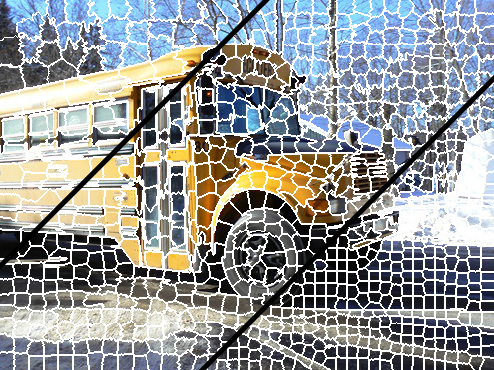
\includegraphics[scale=0.4]{bilder/slic_beispiel}}
\subfigure[Quickshift]{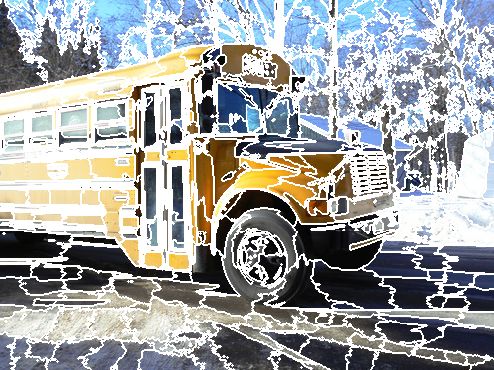
\includegraphics[scale=0.4]{bilder/quickshift_beispiel}}
  \caption[\gls{SLIC} und Quickshift Beispielresultat]{Ein Bus segmentiert über \gls{SLIC} mit jeweils 400, 800 und 1600 Superpixeln (a) sowie über Quickshift mit 600 Superpixeln (b).
  Dabei werden die unterschiedlichen Verfahren zur Generierung von Superpixeln deutlich.
  Wohingegen \gls{SLIC} möglichst quadratische, gleichgroße Superpixel erzeugt, wird die Form der Superpixel von Quickshift größtenteils über die Farbabgrenzungen gesteuert und erzeugt damit sowohl sehr große wie auch sehr kleine Superpixel in allen möglichen Variationen.}
\label{fig:slic_quickshift}
\end{figure}

\subsection{Verfahren}
\label{superpixel_verfahren}

In der Literatur finden sich zahlreiche Verfahren zur Bestimmung einer Superpixelrepräsentation aus einem Bild mit jeweils unterschiedlichen Stärken und Schwächen~\cite{super, slic}.
Zwei beliebte Verfahren, die aufgrund ihrer im Allgemeinen guten Resultate bei geringer Berechnungskomplexität immer wieder zu finden sind, sind der SLIC- sowie der Quickshift-Algorithmus~\cite{slic, super, Gadde, supercnn, Fulkerson}.
Beide Verfahren werden im Folgenden näher vorgestellt.

\paragraph{SLIC}
\label{slic}

Der Superpixelalgorithmus \emph{\gls{SLIC}} ist ein recht einfach gehaltener lokaler \emph{$K$-Means}-Clustering-Ansatz, welcher sich dennoch durch seine Geschwindigkeit, seine Speichereffizienz und insbesondere durch seine erfolgreiche Segmentierung hinsichtlich der Farbabgrenzen seiner Superpixel im Vergleich zu anderen \enquote{State-of-the-Art}-Algorithmen auszeichnet~\cite{slic, Gadde}.

Ein Bild $\gls{B} \in \gls{R}^{H \times C \times 3}$ im \emph{Lab-Farbraum} wird dazu initial in $K \in \gls{N}$ viele Clusterzentren $\ve{c}_k \coloneqq {\left[l_k, a_k, b_k, x_k, y_k\right]}^{\top}$  mit jeweils gleichmäßigem Abstand $S \coloneqq \sqrt{WH/K}$ zerlegt~\cite{slic}.
Daraufhin werden in einem iterativen Prozess die Zugehörigkeiten der Pixel zu ihren jeweiligen Clustern über eine Distanzmetrik $D$ bestimmt und die Clusterzentren entsprechend ihrer neuen Gruppierungen angepasst.
Entgegen der konventionellen $k$-Means-Formulierung werden dabei aber nicht die Distanzen jedes Pixels zu jedem Clusterzentrum berechnet, sondern lediglich für die Pixel, die sich in der Region der Größe $2S \times 2S$ um $\ve{c}_k$ befinden~\cite{slic}.
Dies führt folglich zu einer drastischen Reduzierung der Anzahl an Distanzberechnungen und zu einem effizienteren Algorithmus.
Wurde zu jedem Pixel dessen ähnlichstes Clusterzentrum bestimmt, werden die Zentren über die Durchschnittsbildung all seiner zugehörigen Pixel neu justiert.
Nach einer festgelegten Anzahl an Iterationsschritten (üblicherweise $10$) bricht der Algorithmus schließlich ab~\cite{slic}.
Das gesamte Verfahren ist in Algorithmus~\ref{alg:slic} zusammengefasst.

\begin{algorithm}[t]
\centering
\begin{algorithmic}
  \REQUIRE{} Bild $\gls{B} \in \gls{R}^{H \times W \times 3}$ im Lab-Farbraum, Anzahl der Cluster $K$
  \ENSURE{} Segmentierungsmaske $\gls{Smaske} \in \gls{N}^{H \times W}$
  \STATE{} Initialisiere $K$ Clusterzentren ${\left\{\ve{c}_k\right\}}_{k=1}^K$ mit gleichmäßigem Abstand $S$.
  \STATE{} $\gls{Smaske}_{yx} \leftarrow -1$ für jedes Pixel $\gls{B}_{yx}$ an $\left(x,y\right)$.
  \STATE{} $\ma{D}_{yx} \leftarrow \infty$ für jedes Pixel $\gls{B}_{yx}$ an $\left(x,y\right)$.
  \REPEAT{}
    \FOR{$\ve{c}_k \in {\left\{\ve{c}_k\right\}}_{k=1}^K$}
      \FOR{Pixel $\gls{B}_{yx}$ an $\left(x,y\right)$ in $2S \times 2S$ Region um $\ve{c}_k$}
        \STATE{} Berechne Distanz $D$ zwischen $\ve{c}_k$ und $\gls{B}_{yx}$.
        \IF{$D < \ma{D}_{yx}$}
          \STATE{} $\ma{D}_{yx} \leftarrow D$
          \STATE{} $\gls{Smaske}_{yx} \leftarrow k$
        \ENDIF{}
      \ENDFOR{}
    \ENDFOR{}
    \STATE{} Justiere Clusterzentren ${\left\{\ve{c}_k\right\}}_{k=1}^K$.
  \UNTIL{Endbedingung}
\end{algorithmic}
  \caption[\gls{SLIC}]{\gls{SLIC}-Algorithmus, der eine Segmentierungsmaske $\gls{Smaske} \in \gls{N}^{H \times W}$ in den Ausmaßen des Eingabebildes $\gls{B} \in \gls{R}^{H \times W \times 3}$ über ein lokales $K$-Means-Clustering bei $K$ gleichmäßig verteilten initialen Clusterzentren generiert.}
\label{alg:slic}
\end{algorithm}

Die Distanzmetrik $D$ basiert auf der euklidischen Norm ${\left\|\cdot\right\|}_2$ im fünfdimensionalen Raum ${\left[l,a,b,x,y\right]}^{\top}$ auf den Farben und den Positionen der Pixel \bzw{} der Clusterzentren.
Dabei ergeben sich jedoch Inkonsistenten für unterschiedliche Superpixelgrößen.
Bei großen Superpixeln führt dies zu einer stärkeren Gewichtung der räumlichen Positionen der Superpixel, wohingegen bei kleinen Superpixeln genau das Gegenteil der Fall ist~\cite{slic}.
Es ist daher notwendig, die Distanzen der Positionen $D_S$ und Farben $D_F$ getrennt voneinander zu betrachten und mittels dem Abstand $S$ der initialen Clusterzentren und einer Normalisierungskonstante $F \in \gls{R}$ \bzgl{} der Gewichtung der Farben zu normieren.
Damit ergibt sich $D$ als~\cite{slic}
\begin{equation*}
\begin{split}
  D & \coloneqq \sqrt{{\left(\frac{D_S}{S}\right)}^2 + {\left(\frac{D_F}{F}\right)}^2}\\
  D_S & \coloneqq {\left\|{\left[x, y\right]}^{\top} - {\left[x_k, y_k\right]}^{\top}\right\|}_2\\
  D_C & \coloneqq {\left\|{\left[l, a, b\right]}^{\top} - {\left[l_k, a_k, b_k\right]}^{\top}\right\|}_2.
\end{split}
\end{equation*}
Die Normalisierungskonstante $F$ kann damit auch als Gewichtung zwischen der Form und den Farbabgrenzungen der Superpixel verstanden werden.
Falls $F$ sehr klein gewählt wird, respektieren die Superpixel Farbabgrenzungen besser, aber besitzen im Allgemeinen auch eine eher unreguläre Form~\cite{slic}.

Damit ist \gls{SLIC} ein $\gls{O}\left(WH\right)$ effizienter Algorithmus mit nur zwei frei wählbaren Parametern $K$ und $F$~\cite{slic}.
Viele Anwendungen im Bereich der Bildverarbeitung machen sich daher \gls{SLIC} zu Nutze (\vgl{}~\cite{Gadde, supercnn, super}).
Abbildung~\ref{fig:slic_quickshift} (a) zeigt ein Beispielresultat des \gls{SLIC}-Algorithmus bei unterschiedlich gewählten Anzahlen an Clusterzentren.

\begin{figure}[t]
\centering
\subfigure[\gls{SLIC}]{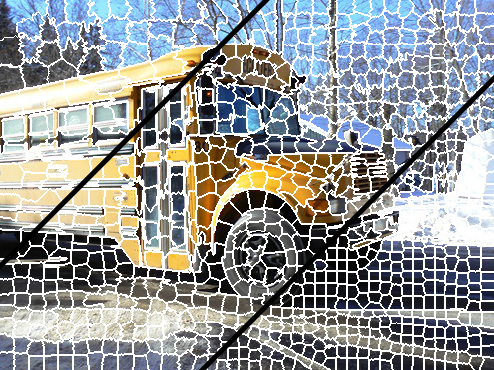
\includegraphics[scale=0.4]{bilder/slic_beispiel}}
\subfigure[Quickshift]{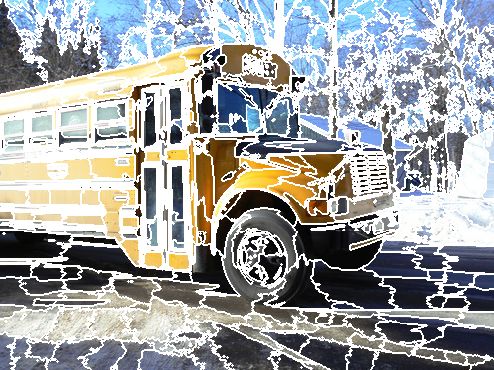
\includegraphics[scale=0.4]{bilder/quickshift_beispiel}}
  \caption[\gls{SLIC} und Quickshift Beispielresultat]{Ein Bus segmentiert über \gls{SLIC} mit jeweils 400, 800 und 1600 Superpixeln (a) sowie über Quickshift mit 600 Superpixeln (b).
  Dabei werden die unterschiedlichen Verfahren zur Generierung von Superpixeln deutlich.
  Wohingegen \gls{SLIC} möglichst quadratische, gleichgroße Superpixel erzeugt, wird die Form der Superpixel von Quickshift größtenteils über die Farbabgrenzungen gesteuert und erzeugt damit sowohl sehr große wie auch sehr kleine Superpixel in allen möglichen Variationen.}
\label{fig:slic_quickshift}
\end{figure}


\paragraph{Quickshift}
\label{quickshift}

\cite{quickshift}
Anwender:~\cite{Fulkerson}.

\paragraph{Weitere Verfahren}
\label{weitere_superpixel_verfahren}

In den letzten Jahren wurden desweiteren zahlreiche eigenvektorbasierte Verfahren zur Bildsegmentierung entwickelt~\cite{super, felzenszwalb}.
Obwohl diese vielversprechende Resultate aufweisen, sind diese jedoch entsprechend langsam um von praktischem Nutzen für die meisten Anwendungen zu sein~\cite{felzenszwalb}.
Andere Algorithmen wiederum zeigen sich als besonders berechnungseffizient, liefern aber dementsprechend unzufriedenstellende Ergebnisse~\cite{felzenszwalb}.
Namenshaft zu erwähnen sei noch die \emph{effiziente graphbasierte Bildsegmentierung} von \citeauthor{felzenszwalb}, die in der Regel unter dem Namen \emph{Felzenszwalb-Segmentierung} bekannt ist~\cite{felzenszwalb}.
Der Algorithmus von \citeauthor{felzenszwalb} zeichnet sich dabei durch seine geringe Berechnungskomplexität aus und versucht gleichzeitig, globale Eigenschaften des Bildes zu erhalten.

As with certain classical clustering methods, our method is based on
selecting edges from a graph, where each pixel corresponds to a node in the graph,
and certain neighboring pixels are connected by undirected edges. Weights on each
edge measure the dissimilarity between pixels. However, unlike the classical methods,
our technique adaptively adjusts the segmentation criterion based on the degree of
variability in neighboring regions of the image~\cite{felzenszwalb}.

Die Felzenszwalb-Segementierung zeigte sich aber in Tests auf einer Reihe von Bildern weniger geeignet, da dessen Parameter für jedes Bild eine spezielle Anpassung benötigen und folglich eine statische Wahl dieser Parameter zu unbrauchbaren Ergebnissen führte.

\subsection{Merkmalsextraktion}
\label{merkmalsextraktion}

Die Darstellung eines Bildes über einen Graphen \gls{G}, der aus einer Superpixelrepräsentation \gls{Smenge} gewonnen wurde, besitzt in der Regel weitaus weniger Knoten im Gegensatz zu der reinen Darstellung des Bildes über eine Gitterrepräsentation.
Die Superpixel \bzw{} die Regionen der Segmentierungsmaske können dabei jedoch die willkürlichsten Formen annehmen und besitzen lediglich die Einschränkung, dass diese stets zusammenhängend sind.
Die Form eines Superpixels muss demnach bestmöglichst eingefangen \bzw{} beschrieben werden können — ein Prozess, der in der Bildverarbeitung als \emph{Merkmalsextraktion} bekannt ist~\cite{momente}.
Ein geeigntes Mittel zur Beschreibung einzelner Objekte in einem segmentierten Bild sind die \emph{Momente}, welche in nicht-zentrierte, translationsinvariante, skalierungsinvariante und rotationsinvariante Momente unterschieden werden~\cite{momente}.

\paragraph{Nicht-zentrierte Momente}
\label{nicht_zentrierte_momente}

Zu der binären Segmentierungsmaske $\gls{Smaske} \in {\left\{0, 1\right\}}^{H \times W}$ sind die \emph{nicht-zentrierten Momente} vom Grad $\left(i+j\right)$, $i,j\in\gls{N}$, definiert als~\cite{momente}
\begin{equation*}
  \gls{M}_{ij} \coloneqq \sum_x^W \sum_y^H x^i y^j \gls{Smaske}_{yx}.
\end{equation*}
Obwohl der Grad eines Moments beliebig hoch gewählt werden kann, so reichen in der Praxis meist wenige Momente niedrigen Grades aus ($\le 3$), um eine Region hinreichend genau zu charakterisieren~\cite{momente}.
Bildeigenschaften, die durch nicht-zentrierte Momente beschrieben werden können, sind unter anderem dessen Fläche über $\gls{M}_{00}$ sowie dessen absoluter Schwerpunkt $\left\{\bar{x}, \bar{y}\right\} = \left\{ \gls{M}_{10}/\gls{M}_{00}, \gls{M}_{01}/\gls{M}_{00}\right\}$~\cite{momente}.

\paragraph{Translationsinvariante (zentrale) Momente}
\label{translationsinvariante_momente}

Nicht-zentrierte Momente sind aufgrund ihrer Berücksichtigung der Position einer Region im Bild meist unerwünscht, sie helfen aber für die weitere Definition von translationsinvarianten Momenten.
Mit Hilfe der absoluten Schwerpunktskoordinaten $\left\{ \bar{x}, \bar{y} \right\}$ können die \emph{translationsinvarianten Momente} über
\begin{equation*}
  \gls{mu}_{ij} \coloneqq \sum_x^W \sum_y^H {\left(x - \bar{x}\right)}^i {\left(y - \bar{y}\right)}^j \gls{Smaske}_{yx}.
\end{equation*}
definiert werden~\cite{momente}.
Sie lassen sich weiterhin direkt aus $\gls{M}_{ij}$ ermitteln.
So gilt \zB{}, dass $\gls{mu}_{00} = \gls{M}_{00}$ oder $\gls{mu}_{11} = \gls{M}_{11} - \bar{x}\gls{M}_{01} = \gls{M}_{11} - \bar{y}\gls{M}_{10}$ (\vgl{}~\cite{momente}).

\paragraph{Skalierungsinvariante Momente}
\label{skalierungsinvariante_zentrierte_momente}

Für $i+j \geq 2$ können desweiteren die \emph{skalierungsinvarianten Momente} $\gls{eta}_{ij}$ konstruiert werden, die invariant \bzgl{} Skalierung und Translation sind.
Dafür wird das entsprechende translationsinvariante Moment $\gls{mu}_{ij}$ durch die entsprechende Fläche $\gls{M}_{00}$ \bzw{} $\gls{mu}_{00}$ des Segments geteilt, \dhe{}~\cite{momente}
\begin{equation*}
  \gls{eta}_{ij} = \frac{\gls{mu}_{ij}}{\gls{mu}_{00}^{\left(1+\left(i+j\right)/2\right)}}.
\end{equation*}

\paragraph{(Rotationsinvariante) Hu-Momente}
\label{rotationsinvariante_momente}

\citeauthor{Hu} verwendet eine nichtlineare Kombination der skalierungsinvarianten Momente bis zum Grad $3$, um aus ihnen zusätzlich eine Rotationsinvarianz zu gewinnen~\cite{Hu, momente}.
Daraus ergeben sich sieben \emph{rotationsinvariante Momente} oder \emph{Hu-Momente}.
\begin{equation*}
\begin{split}
  \gls{hu}_1 & = \gls{eta}_{20} + \gls{eta}_{02}\\
  \gls{hu}_2 & = {\left(\gls{eta}_{20} - \gls{eta}_{02}\right)}^2 + {\left(2\gls{eta}_{11}\right)}^2\\
  \gls{hu}_3 & = {\left(\gls{eta}_{30} - 3\gls{eta}_{12}\right)}^2 + {\left(3\gls{eta}_{21} - \gls{eta}_{03}\right)}^2\\
  \gls{hu}_4 & = {\left(\gls{eta}_{30} + \gls{eta}_{12}\right)}^2 + {\left(\gls{eta}_{21} + \gls{eta}_{03}\right)}^2\\
  \gls{hu}_5 & = \left(\gls{eta}_{30} - 3\gls{eta}_{12}\right)\left(\gls{eta}_{30} + \gls{eta}_{12}\right) \left({\left(\gls{eta}_{30} + \gls{eta}_{12}\right)}^2 - 3{\left(\gls{eta}_{21} + \gls{eta}_{03}\right)}^2\right)\\
  & + \left(3\gls{eta}_{21} - \gls{eta}_{03}\right)\left(\gls{eta}_{21} + \gls{eta}_{03}\right) \left(3{\left(\gls{eta}_{30} + \gls{eta}_{12}\right)}^2 - {\left(\gls{eta}_{21} + \gls{eta}_{03}\right)}^2\right)\\
  \gls{hu}_6 & = \left(\gls{eta}_{20} - \gls{eta}_{02}\right)\left({\left(\gls{eta}_{30} + \gls{eta}_{12}\right)}^2 - {\left(\gls{eta}_{21} + \gls{eta}_{03}\right)}^2\right) + 4\gls{eta}_{11}\left(\gls{eta}_{30} + \gls{eta}_{12}\right)\left(\gls{eta}_{21} + \gls{eta}_{03}\right)\\
  \gls{hu}_7 & = \left(3\gls{eta}_{21} - \gls{eta}_{03}\right)\left(\gls{eta}_{30} + \gls{eta}_{12}\right) \left({\left(\gls{eta}_{30} + \gls{eta}_{12}\right)}^2 - 3{\left(\gls{eta}_{21} + \gls{eta}_{03}\right)}^2\right)\\
  & + \left(\gls{eta}_{03} - 3\gls{eta}_{12}\right)\left(\gls{eta}_{21} + \gls{eta}_{03}\right) \left(3{\left(\gls{eta}_{30} + \gls{eta}_{12}\right)}^2 - {\left(\gls{eta}_{21} + \gls{eta}_{03}\right)}^2\right)
\end{split}
\end{equation*}

\paragraph{Interpretation}
\label{interpretation_momente}

\todo{kovarianzmatrix \bzw{} inertia tensor}

\paragraph{Weitere Merkmale}
\label{weitere_merkmale}

\paragraph{Caching}
\label{Caching}

\cite{Siedhoff}

